% Fig 1: SecurePath Framework Overview
% Compile with: pdflatex fig1_framework.tex
\documentclass[tikz,border=8pt]{standalone}
\usepackage{amsmath}
\usetikzlibrary{
  positioning,
  arrows.meta,
  shapes.geometric,
  shapes.multipart,
  fit,
  backgrounds,
  calc
}

\definecolor{stage1bg}{RGB}{235,245,255}
\definecolor{stage2bg}{RGB}{255,248,235}
\definecolor{stage3bg}{RGB}{240,255,240}
\definecolor{blue1}{RGB}{30,100,180}
\definecolor{orange1}{RGB}{200,120,20}
\definecolor{green1}{RGB}{30,140,80}
\definecolor{red1}{RGB}{180,40,40}
\definecolor{gray1}{RGB}{100,100,100}

\begin{document}
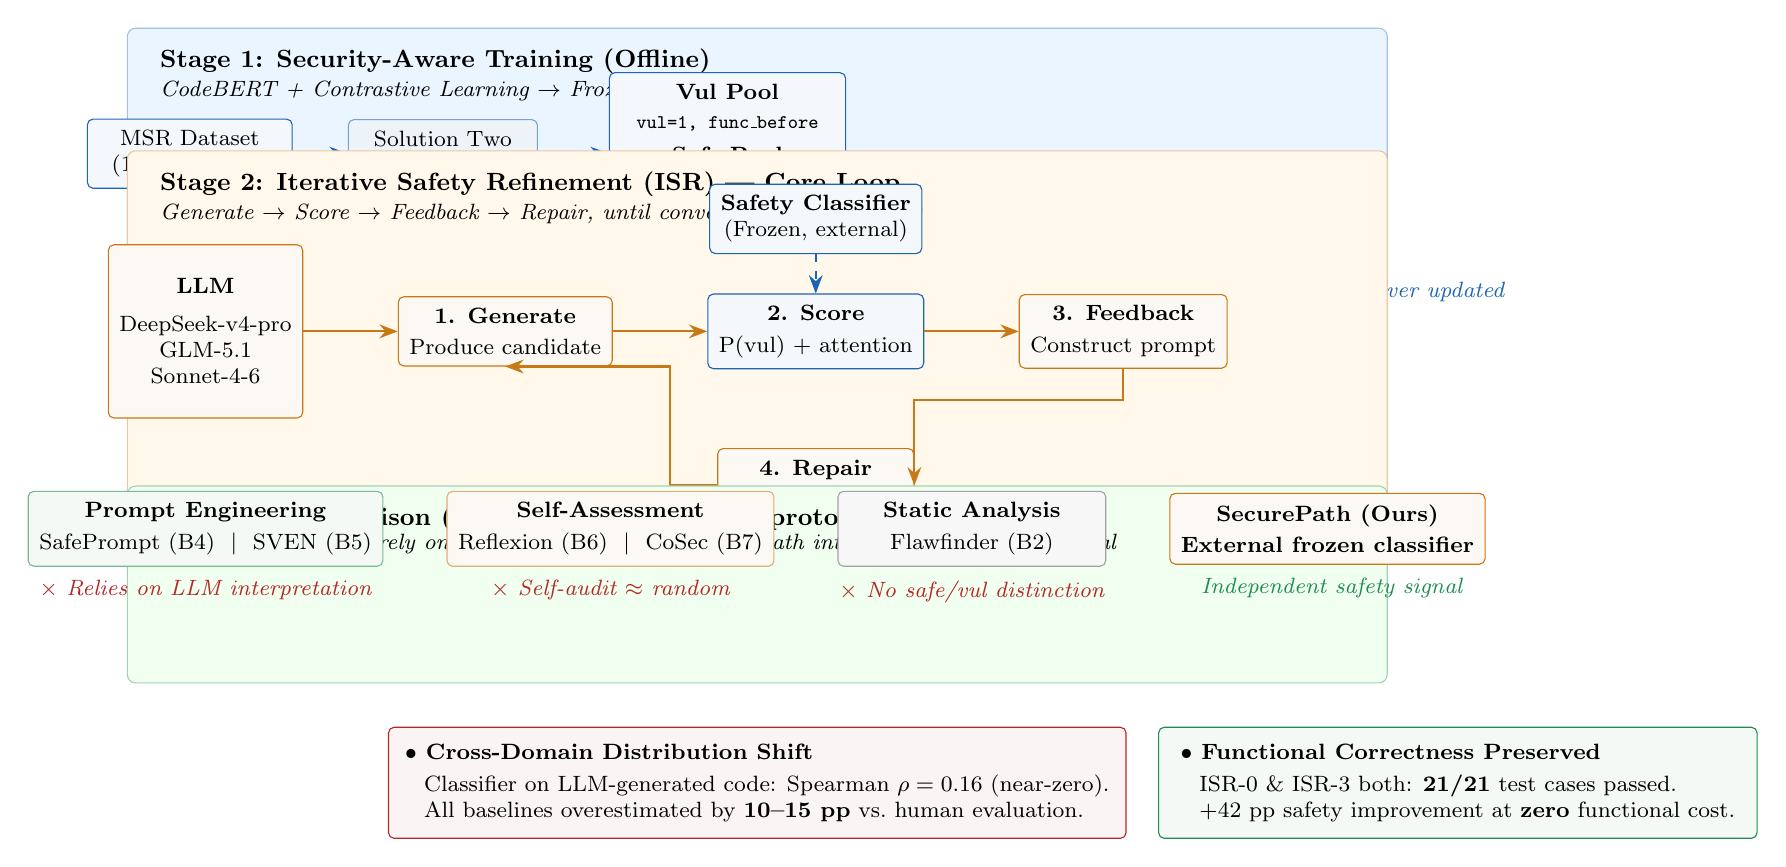
\begin{tikzpicture}[
  >=Stealth,
  node distance=0.6cm and 0.6cm,
  % Box styles
  box/.style={
    draw=black, fill=white, rounded corners=2pt,
    minimum height=0.7cm, align=center,
    font=\footnotesize, inner sep=4pt
  },
  boxblue/.style={box, draw=blue1, fill=blue1!5},
  boxorange/.style={box, draw=orange1, fill=orange1!5},
  boxgreen/.style={box, draw=green1, fill=green1!5},
  boxred/.style={box, draw=red1, fill=red1!5},
  boxgray/.style={box, draw=gray1, fill=gray1!5},
  % Arrow
  arr/.style={->, >=Stealth, thick},
  % Panel background
  panel/.style={rounded corners=3pt, inner sep=7pt},
]

% ============================================================
% PANEL 1: Security-Aware Training
% ============================================================
\node[panel, fill=stage1bg, draw=blue1!40,
      minimum width=16.0cm, minimum height=4.3cm] (P1) at (0,0) {};

\node[font=\bfseries\small, anchor=north west] at ([xshift=0.3cm, yshift=-0.15cm]P1.north west)
  {Stage 1: Security-Aware Training (Offline)};
\node[font=\footnotesize\itshape, anchor=north west] at ([xshift=0.3cm, yshift=-0.55cm]P1.north west)
  {CodeBERT + Contrastive Learning $\rightarrow$ Frozen Safety Classifier};

% Row 1: Data flow
\node[boxblue, minimum width=2.6cm] (msr) at ([xshift=0.8cm, yshift=-1.6cm]P1.north west)
  {MSR Dataset\\(188,636 funcs)};
\node[box, draw=blue1!60, fill=blue1!8, minimum width=2.4cm, right=0.7cm of msr] (sol2)
  {Solution Two\\Preprocessing};
\node[boxblue, minimum width=3.0cm, right=0.9cm of sol2] (pools)
  {\textbf{Vul Pool}\\[1pt] {\scriptsize\texttt{vul=1, func\_before}}\\[3pt]
   \textbf{Safe Pool}\\[1pt] {\scriptsize\texttt{vul=0, func\_before}}\\[1pt]
   {\scriptsize\texttt{vul=1, func\_after}}};

\draw[arr, blue1] (msr) -- (sol2);
\draw[arr, blue1] (sol2) -- (pools);

% Row 2: Training pipeline
\node[boxblue, minimum width=2.8cm, below=0.7cm of sol2] (codebert)
  {CodeBERT-base\\(125M, frozen)\\[2pt] InfoNCE Contrastive};
\node[boxblue, minimum width=2.8cm, right=0.9cm of codebert] (attn)
  {AttentionPooling\\(590K)\\[2pt] + MLP Classifier\\(230K)};
\node[boxorange, minimum width=2.8cm, right=0.9cm of attn] (clsout)
  {\textbf{Frozen Classifier}\\[3pt] {\footnotesize F1=0.896~~AUC=0.953}\\[1pt]
   {\footnotesize Per-CWE F1 $>$ 0.88}};

\draw[arr, blue1] (pools.south) -- ++(0,-0.25) -| (codebert.north);
\draw[arr, blue1] (codebert) -- (attn);
\draw[arr, blue1] (attn) -- (clsout);

% Annotation
\node[font=\footnotesize\itshape, text=blue1, anchor=west] at ([xshift=0.3cm]clsout.east)
  {Trained once,\\never updated};

\node[font=\footnotesize\bfseries, text=green1] at ([yshift=-0.2cm]pools.south)
  {$\checkmark$ No feature collapse};

% ============================================================
% PANEL 2: ISR Loop
% ============================================================
\node[panel, fill=stage2bg, draw=orange1!40,
      minimum width=16.0cm, minimum height=5.5cm] (P2)
  at (0, -2.15cm |- P1.south) {};

\node[font=\bfseries\small, anchor=north west] at ([xshift=0.3cm, yshift=-0.15cm]P2.north west)
  {Stage 2: Iterative Safety Refinement (ISR) --- Core Loop};
\node[font=\footnotesize\itshape, anchor=north west] at ([xshift=0.3cm, yshift=-0.55cm]P2.north west)
  {Generate $\rightarrow$ Score $\rightarrow$ Feedback $\rightarrow$ Repair, until convergence (max 5 iter.)};

% Left: LLM box
\node[boxorange, minimum width=2.4cm, minimum height=2.2cm] (llm) at ([xshift=1.0cm, yshift=-2.3cm]P2.north west)
  {\textbf{LLM}\\[4pt] DeepSeek-v4-pro\\GLM-5.1\\Sonnet-4-6};

% Cycle: 4 nodes
%   Generate -- Score -- Feedback
%                |         |
%              Repair <----+
%                |
%           back to Generate
\node[boxorange, minimum width=2.2cm, right=1.2cm of llm] (generate)
  {\textbf{1. Generate}\\[2pt] \footnotesize Produce candidate};
\node[boxblue, minimum width=2.2cm, right=1.2cm of generate] (score)
  {\textbf{2. Score}\\[2pt] \footnotesize P(vul) + attention};
\node[boxorange, minimum width=2.2cm, right=1.2cm of score] (feedback)
  {\textbf{3. Feedback}\\[2pt] \footnotesize Construct prompt};
\node[boxorange, minimum width=2.2cm, below=1.0cm of score] (repair)
  {\textbf{4. Repair}\\[2pt] \footnotesize LLM regenerates};

% Cycle arrows
\draw[arr, orange1] (llm) -- (generate);
\draw[arr, orange1] (generate) -- (score);
\draw[arr, orange1] (score) -- (feedback);
\draw[arr, orange1] (feedback.south) -- ++(0,-0.4) -| (repair.east);
\draw[arr, orange1] (repair.west) -- ++(-0.6,0) |- (generate.south);

% Classifier above Score
\node[boxblue, minimum width=2.4cm, above=0.5cm of score] (clsbox)
  {\textbf{Safety Classifier}\\(Frozen, external)};
\draw[arr, blue1, dashed] (clsbox) -- (score);

% ISR variants below repair
\node[boxgray, minimum width=3.6cm, below=0.8cm of repair, font=\footnotesize] (isr_variants)
  {\textbf{Feedback Variants}\\[2pt]
   ISR-1 (Generic) ~$\mid$~ ISR-2 (+Attention) ~$\mid$~ ISR-3 (+Spec)};

% Effect arrow
\node[font=\footnotesize\bfseries] (hlabel) at ([xshift=0.6cm, yshift=0.35cm]P2.south west) {Human SAFE:};
\node[boxred, font=\footnotesize\bfseries, minimum width=1.3cm, right=0.3cm of hlabel] (rate0) {45.5\%};
\draw[arr, orange1, line width=1.5pt] ([xshift=0.2cm]rate0.east) -- ++(2.0cm,0)
  node[midway, above, font=\footnotesize\bfseries] {ISR};
\node[boxgreen, font=\footnotesize\bfseries, minimum width=1.3cm, right=2.3cm of rate0] (rate3) {87.5\%};
\node[font=\footnotesize\bfseries, text=green1, right=0.15cm of rate3] {+42 pp};

% ============================================================
% PANEL 3: Baselines
% ============================================================
\node[panel, fill=stage3bg, draw=green1!40,
      minimum width=16.0cm, minimum height=2.5cm] (P3)
  at (0, -2.75cm |- P2.south) {};

\node[font=\bfseries\small, anchor=north west] at ([xshift=0.3cm, yshift=-0.15cm]P3.north west)
  {Baseline Comparison (Same human evaluation protocol)};
\node[font=\footnotesize\itshape, anchor=north west] at ([xshift=0.3cm, yshift=-0.5cm]P3.north west)
  {All existing methods rely on LLM self-assessment; SecurePath introduces an \textbf{external} signal};

% Three baseline boxes
\node[box, minimum width=3.4cm, minimum height=0.9cm,
      draw=green1!60, fill=green1!5, font=\footnotesize] (b1) at ([xshift=1.0cm, yshift=-0.55cm]P3.north west)
  {\textbf{Prompt Engineering}\\[2pt] SafePrompt (B4) ~$\mid$~ SVEN (B5)};

\node[box, minimum width=3.4cm, minimum height=0.9cm,
      draw=orange1!60, fill=orange1!5, font=\footnotesize, right=0.8cm of b1] (b2)
  {\textbf{Self-Assessment}\\[2pt] Reflexion (B6) ~$\mid$~ CoSec (B7)};

\node[box, minimum width=3.4cm, minimum height=0.9cm,
      draw=gray1!60, fill=gray1!5, font=\footnotesize, right=0.8cm of b2] (b3)
  {\textbf{Static Analysis}\\[2pt] Flawfinder (B2)};

\node[boxorange, minimum width=3.4cm, minimum height=0.9cm,
      font=\footnotesize\bfseries, right=0.8cm of b3] (innov)
  {\textbf{SecurePath (Ours)}\\[2pt] External frozen classifier};

% Red X annotations
\node[font=\footnotesize\itshape, text=red1, below=0.05cm of b1.south, anchor=north]
  {$\times$ Relies on LLM interpretation};
\node[font=\footnotesize\itshape, text=red1, below=0.05cm of b2.south, anchor=north]
  {$\times$ Self-audit $\approx$ random};
\node[font=\footnotesize\itshape, text=red1, below=0.05cm of b3.south, anchor=north]
  {$\times$ No safe/vul distinction};
\node[font=\footnotesize\itshape, text=green1, below=0.05cm of innov.south, anchor=north]
  {$\checkmark$ Independent safety signal};

% ============================================================
% CALLOUT BOXES
% ============================================================
\node[boxred, minimum width=7.8cm, minimum height=1.2cm,
      below=0.55cm of P3, font=\footnotesize, align=left, inner sep=6pt] (callout1)
  {\textbf{$\bullet$ Cross-Domain Distribution Shift}\\[2pt]
   \hspace{4pt} Classifier on LLM-generated code: Spearman $\rho = 0.16$ (near-zero).\\
   \hspace{4pt} All baselines overestimated by \textbf{10--15 pp} vs.\ human evaluation.};

\node[boxgreen, minimum width=7.6cm, minimum height=1.2cm,
      right=0.4cm of callout1, font=\footnotesize, align=left, inner sep=6pt] (callout2)
  {\textbf{$\bullet$ Functional Correctness Preserved}\\[2pt]
   \hspace{4pt} ISR-0 \& ISR-3 both: \textbf{21/21} test cases passed.\\
   \hspace{4pt} +42 pp safety improvement at \textbf{zero} functional cost.};

\end{tikzpicture}
\end{document}
